\chapter{Der neue Ansatz} \label{der-neue-ansatz}

\section{Steigende Robustheit durch TypeScript}

% Mehr Projekte nutzen TypeScript => sind bereits was Typing angeht robust
% TypeScript ist auch in fast allen IDEs integriert, also wird fast von jedem genutzt.
TypeScript verfügt, im Gegensatz zu JavaScript, über statische Typisierung. Dank der statischen Typisierung sind Operationen wie \textit{Go to Definition} und \textit{Go to Implementations} der Entwicklungsumgebungen (IDE) möglich. Diese Eigenschaften reduzieren Fehler im Zusammenhang mit falschen Typen erheblich. Wie in \ref{fig:js-und-ts-nutzung-2018-2024} abgebildet, wird TypeScript von immer mehr Entwicklern genutzt, während die JavaScript Nutzung abnimmt. \ref{fig:js-und-ts-nutzung-2018-2024} beinhaltet die tatsächliche Nutzung von TS nicht. Der TypeScript Compiler (tsc) ist in den meisten modernen IDEs, wie Visual Studio Code und den JetBrains IDEs wie IntelliJ IDEA und WebStorm integriert. Dies führt dazu, dass man auch beim JavaScript Code einige Vorteile von TypeScript bekommt.\cite{typeScriptDocumentary}

\begin{figure}[H]
  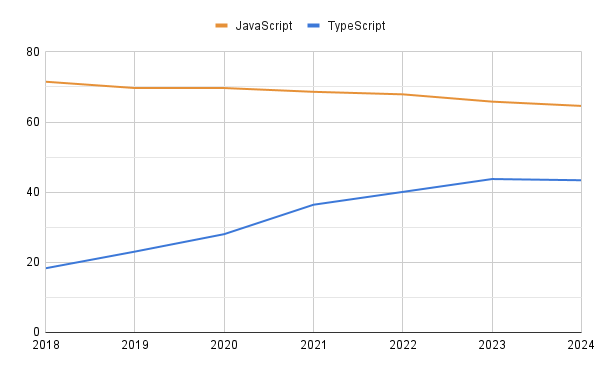
\includegraphics[width=1\textwidth]{js-und-ts-nutzung-2018-2024.png}
  \caption{Prozentuale Nutzung von JavaScript und TypeScript unter professionellen Entwicklern von 2018 bis 2024}
  \label{fig:js-und-ts-nutzung-2018-2024}
\end{figure}

% Um Implementierungsfehler zu vermeiden => Transitions robuster machen

\section {Unzureichende Robustheit in State-Management}

Der TypeScript-Faktor macht Webapplikationen, somit auch State-Management auf Typ-Ebene robuster und weniger fehleranfällig. Allerdings ist es für die Applikation immer noch möglich in einem falschen Zustand zu sein. Gegeben sei ein eine Redux Store, der für das Speichern von einer Liste von \textit{items} zuständig ist. Definiert wird der Store wie folgt:

\begin{lstlisting}
  type FetchAction = {
    type: 'fetch'
  }

  type FetchSuccessfulAction = {
    type: 'fetch-successful',
    payload: Array<any>
  }

  type FetchFailedAction = {
    type: 'fetch-failed',
    payload: Error
  }

  type Action = FetchAction | 
    FetchSuccessfulAction |
    FetchFailedAction

  function reducer(
    state = { items: 'not-fetched' }, 
    action: Action
  ) {
    switch (action.type) {
      case 'fetch':
        return {
          ...state,
          items: 'fetching'
        }
      case 'fetch-successful':
        return {
          ...state,
          items: action.payload
        }
      case 'fetch-failed':
        return {
          ...state,
          items: action.payload
        }
      default:
        return state
    }
  }
  
  const store = createStore(reducer)
\end{lstlisting}

Es ist erlaubt, die \textit{FetchSuccessfulAction} Aktion zu versenden, ohne voher die \textit{Fetch} Aktion versendet zu haben. Das heißt \textit{items} wurden erfolgreich abrufen, ohne die Anfrage zuvor gemacht zuhaben. Seitens Redux ist das Versenden einer Aktion immer, unbeachtet des aktuellen Zustandes, erlaubt. Dieser Faktor spricht gegen die Nachvollziehbarkeit und gilt für alle populäre SM Lösungen.

\section {Robustere Zustandsübergänge}

Es wird vorgeschlagen Übergänge wie bei einem DFA für den Store zu definieren und den Zustandswechsel wie eine Übergangsfunktion zu behandeln. Dabei werden die Zustände, im oberen Fall \textit{'not-fetched'}, \textit{'fetching'}, \textit{Error} und und \textit{Array<any>}, als Zustände des DFAs behandelt. Restliche Eigenschaften des Quintupels eines DFAs werden hierbei ignoriert.

Um die Übergangsfunktion zu definieren, wird eine Liste aller Aktionen benötigt, die bei einem bestimmten Zustand erlaubt sind. Ein Problem hierbei ist allerdings, dass die Identifizierbarkeit der einzelnen Zustände nicht garantiert ist.
Abweichend von DFAs, sind die Zustände in Webapplikationen nicht immer serialisierbar. Nicht serialisierbare Objekte sind nicht immer identifizierbar. Im oberen Beispiel, sind die Zustände \textit{'not-fetched'} und \textit{'fetching'} vom Type String und somit serialisierbar, allerdings sind die restlichen Zustände nicht serialisierbar (Zustand vom Typ Error und Array<any>). Um dieses Problem zu umgehen, wird eine \textit{Kondition Funktion} emfohlen, um zwischen verschiedenen Zuständen zu unterscheiden. Sie akzeptiert als Paramter den aktuellen Zustand und gibt ein Boolean zurück.

\begin{lstlisting}
type Condition<S> = (state: S) => boolean
\end{lstlisting}

% ODER SO:
% Sei $S$ die Menge aller Zustände und $B := \{true, false\}$, dann wird die \textit{Konfition FunKtion} wie folgt definitiert:
% $f(s) = b | s \in S \land b \in B$

Mit dieser Funktion kann jeder Zustand identifiziert werden. Bei JavaScript Klassen, kann der \textit{instanceof} Operator genutzt werden, um auf die Instanz einer Klasse wie \textit{Error} zu prüfen.\cite{jsInstanceofOperator} Desweiteren, können bei Objekten auf eindeutige Eigenschaften, wie die Präzens eines Feldes per \textit{in} Operator geprüft werden.\cite{jsInOperator} Bei Arrays kann die \textit{Array.isArray} Funktion verwendet werden.\cite{jsIsArray} Durch die Kombinition dieser und weiteren Funktionen und Operatoren können weitere Datentypen und Fälle identifiziert werden.

Jeder Übergang wird mit einer \textit{Validierungsfunktion} validiert. Diese prüft auf die Gültigkeit eines Übergangs und wirft einen Laufzeitfehler bei ungültigen Aufrufen. Falls der Übergang gültig ist, wirft sie keine  Fehler und der Zustandswechsel kann stattfinden. Der Laufzeitfehler sorgt dafür, dass der ungültige Aufruf berichtet wird und sich nicht zu einem langlebigen Bug entwicklen kann.